
\documentclass[10pt]{article}

\usepackage{amsmath}
\usepackage{amssymb}

\usepackage{graphicx}

\usepackage{cite}

\usepackage{color}


\topmargin 0.0cm
\oddsidemargin 0.5cm
\evensidemargin 0.5cm
\textwidth 16cm
\textheight 21cm

\usepackage[labelfont=bf,labelsep=period,justification=raggedright]{caption}

\bibliographystyle{unsrt}

\makeatletter
\renewcommand{\@biblabel}[1]{\quad#1.}
\makeatother


\date{}

\pagestyle{myheadings}
\usepackage{bussproofs}
\usepackage[all]{xy}
\usepackage{subcaption}
\usepackage[backref]{hyperref}
\hypersetup{colorlinks=true,
linkcolor=[rgb]{.67 .27 .27},
citecolor=[rgb]{.09 .29 .54},
urlcolor=[rgb]{.09 .29 .54}}
\usepackage[table]{xcolor}
\usepackage{rotating}
\usepackage[colorinlistoftodos]{todonotes}
\usepackage{verbatim}

%-----------------------------
\usepackage{bm}
%\usepackage[toc]{multitoc}
\usepackage{titletoc}
\usepackage{etoolbox}
\usepackage{amssymb}
\usepackage{amsmath}
\usepackage{amsthm}
\usepackage[all]{xy}
\usepackage{tikz}
\usepackage{tikz-cd}

%-----------------------------
% Theorem environments.
%-----------------------------
\theoremstyle{plain}
\newtheorem{theorem}[subsection]{Theorem}
\newtheorem{proposition}[subsection]{Proposition}
\newtheorem{lemma}[subsection]{Lemma}

\theoremstyle{definition}
\newtheorem{definition}{Definition}
\newtheorem{example}[subsection]{Example}
\newtheorem{exercise}[subsection]{Exercise}
\newtheorem{situation}[subsection]{Situation}

\theoremstyle{remark}
\newtheorem{remark}[subsection]{Remark}
\newtheorem{remarks}[subsection]{Remarks}

%-----------------------------
% Macros
%-----------------------------

\def\Hom{\mathop{\rm Hom}\nolimits}

%-----------------------------

\usepackage{latexsym}
\usepackage{stmaryrd}

\setcounter{tocdepth}{4}
\setcounter{secnumdepth}{0}


\renewcommand*{\figureautorefname}{Fig.}
\renewcommand*{\equationautorefname}{Eq.}
\renewcommand*{\tableautorefname}{Table}
\renewcommand*{\sectionautorefname}{Sec.}
\renewcommand*{\subsectionautorefname}{Sec.}


\begin{document}

\let\ref\autoref

\pagenumbering{gobble}
% \tableofcontents
% \listoffigures
\pagebreak
\pagenumbering{arabic}

\begin{flushleft}
{\Large
\textbf{A minimal language for functional closure and the origin of evolvability}
}
\\
Cameron Smith$^{1, \ast}$
\\
\bf{1} Department of Systems and Computational Biology, Albert Einstein College of Medicine, Bronx, NY, USA
\\
$\ast$ E-mail: cameron.smith@med.einstein.yu.edu
\end{flushleft}

% \listoftodos

% comment to omit numbering of sections
\setcounter{secnumdepth}{4}

\section{Summary}
Evolvability is the property of a system that specifies its capacity to have its architecture shaped by natural selection~\cite{Wagner2008b}. This is one of the key properties that is considered to distinguish living systems from non-living ones. On one hand, this property obviously implies of a system that its architecture is capable of change. However, from an information theoretic, and thus thermodynamic, perspective, it may be considered that the mechanism capable of maintaining an identity in the form of memory via error correction or repair is a much more difficult necessary condition to be satisfied~\cite{Gacs2001}. Here we argue that one necessary precondition for evolvability and thus for evolutionary processes, which has been previously suggested to be a definitive characteristic of life~\cite{Rosen1972,Rosen1991,Zafiris2012,Mossio2009,Letelier2006} is what we refer to as ``functional closure''. We consider formal languages capable of expressing the functional closure property and then ask, among all languages capable of its expression, which is the language of minimal expressive power?  We do not answer this question conclusively, but discuss potential lower and upper bounds that point to consideration of the conceptual space between the simply-typed and type-free lambda calculi~\cite{Barendregt1985}. We describe how investigation of languages with expressive power lying between these two extremes may be undertaken using tools of modern categorical logic~\cite{Crole1994a,Awodey2006}.

\section{Introduction}
In recent years the abilities to chemically synthesize and transplant genomes to alter organismal identity \cite{Gibson2010} and to execute simulations of the life cycle of a single-celled organism \cite{Karr2012} by collecting measurements of a large number of parameter values conveying detailed information about its underlying processes and integrating them into presumably analogous coupled algorithmic processes have been demonstrated. These capacities and the technologies that may result from them add to the mounting pressure underlying the existence of integrative subfields like systems biology to ask increasingly broad questions about biological systems. In an effort to synthesize knowledge from an enormous number of empirical investigations, is it possible to characterize abstract properties that are necessary, and eventually sufficient, to determine a process capable of generating organisms \emph{de novo} from chemistry? Answering questions like this one are crucial for clarifying hypotheses germane to understanding what is required in order to explain the origin and distinguishing characteristics of life and thus the origin and nature of evolutionary processes.

Very few biologists or other scientists dispute that evolution is the most fundamental organizing concept that is considered to be part of biology itself. In this light, it may seem surprising that not even more effort than has already been exerted is invested in clarifying and formalizing increasingly detailed conceptions of its origins and operation. In order to understand biological systems, it will be necessary to address the question: What are the necessary enabling conditions that make biological evolution possible? The synthesis of some potential answers to this question may clarify a path toward defining a sufficient collection of preconditions for evolutionary processes to take flight.

One such candidate precondition for evolutionary processes, which has been previously suggested to be a ``defining characteristic of life''\cite{Rosen1972,Rosen1978,Rosen1985,Rosen1991}, is \emph{functional closure}. This condition or property attempts to formalize the intuition that the living state is associated with mathematical closure with respect to the generators of metabolic processes necessary for collections of such chemical transformations to become associated to biological organisms. In order to define this term and its context, we begin with an algebraic and associated diagrammatic framework for modelling prototypical biochemical reaction networks. We give an example of a functionally closed network architecture in this framework and then proceed to ask: What is the \emph{minimally complex} formal language capable of expressing the functional closure property?

The concept of linguistic expressive power from computer science helps to motivate this question \cite{Felleisen1991}. \emph{Expressive power} is used both heuristically and formally to rank order models of computation, programming languages, and their associated logics with respect to one another and with respect to so-called \emph{natural language}. Roughly speaking, an increased level of theoretical expressive power of a language correlates with its ability to express more complex or sophisticated ideas. One might ask why it is not always desirable to work within the extant language containing the highest possible expressive power. One reason to consider less expressive languages is that important questions about them can be answered algorithmically with appropriate computing resources in a practical amount of time and memory, whereas the same questions posed of languages with more expressive power are known not to be able to be answered by such means\cite{Hopcroft2007}. Thus, identifying a \emph{minimal} language capable of expressing the necessary conditions for the origin of evolutionary processes is directly germane to the continuing development of exquisitely detailed models of organisms beginning at the molecular level as they are refined and embedded into equally detailed multi-level models of populations, communities, and ecosystems.

In this light, we can refine the question, ``Is there a formal language capable of expressing the functional closure property?'' by adjoining the follow-up question, ``If so, among those that are, which is the language of minimal expressive power?'' We begin to address the first question by attempting to state and interpret the functional closure property in terms of an abstract algebraic language that describes relationships among mathematical functions. From a naive perspective, the definition of functional closure violates the fundamental assumption of typing discipline that is commonly associated to the use of this language. The functional closure property, can nevertheless be interpreted in terms of a standard model of computation that is theoretically more expressive: the untyped or type-free $\lambda$-calculus \cite{Mossio2009}. We find that the originally attempted algebraic interpretation, itself associated to the so-called simply-typed form of the $\lambda$-calculus, of functional closure can be recovered, albeit it in a more complicated form, via the typical category theoretic semantics for the untyped $\lambda$-calculus \cite{Scott1980,Barendregt1985,Abramsky1995}.

Although the untyped $\lambda$-calculus and its associated category theoretic semantics are capable of expressing the functional closure property, this method has at least two problems. One is that the untyped $\lambda$-calculus is, speaking relative to other languages of its kind, (too) highly expressive as it is indeed capable of general recursion. The second is that the untyped $\lambda$-calculus is capable of expressing functional closure in a trivial way via something as simple as an identity function. A simple solution might seem to pass to the simply-typed $\lambda$-calculus, of which the untyped $\lambda$-calculus has been argued to be a special case. However, as a result of the analogous category theoretic semantics for the simply-typed $\lambda$-calculus, attempting to do so brings us back to the original category theoretic interpretation of the diagram expressing the functional closure property that we demonstrated to be type-theoretically inconsistent.

This circularity suggests that potential answers to the second question regarding the minimal expressive power retaining the capacity for functional closure may be found in various extensions of the simply-typed $\lambda$-calculus (some of these may be found on the seven additional vertices of Barendregt's lambda cube \cite{Barendregt1985}). We discuss these issues with respect to the goal of identifying a language of minimal expressive power capable of representing or \emph{approximating} the functional closure property. The latter may ultimately be more important in light of the fact that the functional closure property in its present formulation may be too strong to be relevant to the constraints inherent to chemistry and thus biology in our universe. The conclusion then is that the intuitive characterization of functional closure that is associated to autopoiesis, has always been conceived in a manner that is too strong from a logical perspective to serve as a basis for evolutionary processes. In order to recover a relevance to chemistry and biology, the conception of functional closure thus likely requires weakening in at least one if not several directions.


\section{Metabolism-oriented abstraction of biological organization}\label{sec:metabolismabstraction}
\begin{figure}
\begin{center}
\noindent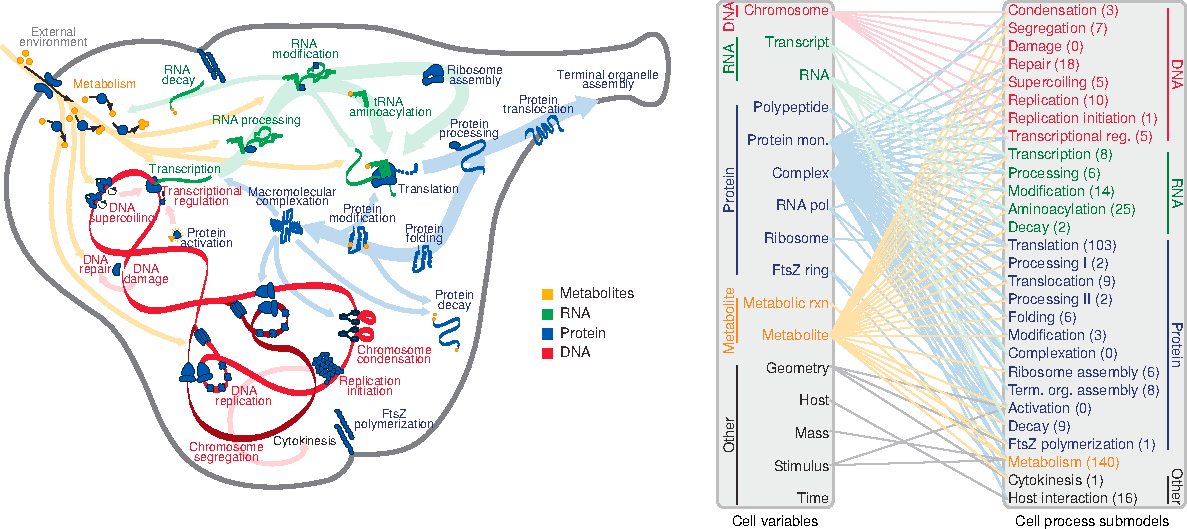
\includegraphics[width=0.95\columnwidth]{fig/cellprocessesdiagram.pdf}
\end{center}
\caption[Cell model]{A schematic depiction of some processes underlying a prokaryotic organism (\emph{M. genitalium}) used in developing an individual life-cycle computational model. Reused with permission from \cite{Karr2012}.}
\label{fig:cellprocess}
\end{figure}
Many salient features of biological organization at the level of a simple parasitic single-celled organism have recently been encapsulated in a unified computational model of the life-cycle of such a cell. In particular, this model tracks 16 important cell-level variables that each depend on a specified subset of 28 cellular processes. \ref{fig:cellprocess} shows a schematic depicting the interrelationships between these processes specified in the context of this model.

From an energetic, and thus physical, perspective, metabolic processes like the citric acid cycle (see \ref{fig:ctacyc}) are certainly fundamental to the existence and persistence of all evolvable systems. As shown in \ref{fig:cellprocess}, metabolic processes form the connection between the dual components induced by considering cells as systems in the first place: the internal and the external environment. Moreover, it has been argued that metabolic processes form the basis or atomic level in a hierarchy of cellular processes. From this point of view, the complex regulatory networks involving small molecules, DNA, proteins and other molecular types are viewed as subservient to and layered atop core metabolic processes. Moreover, metabolic processes may be viewed as causally prior to the origin of evolution \cite{Braakman2012,Braakman2012a}.

These facts regarding the fundamental nature of metabolic networks motivate the attempt to model metabolism abstractly in order to characterize and parse its essential properties from those that may represent unnecessary historical contingency. There are several existing formalisms for constructing dynamical models of metabolic processes. However, these do not attempt to explain how metabolic processes originated or how they are maintained by complex networks of molecular interactions that are themselves considered to be only indirectly related to metabolic processes.

Robert Rosen suggested a formalism for metabolic networks that does attempt to abstractly incorporate the interrelationships between metabolic networks and the the associated regulatory networks involving interactions among DNA, RNA, and proteins \cite{Rosen1972,Rosen1991}. In some sense, metabolic processes must be able to intrinsically construct at least some of their own causal antecedents. The justification for stating ``at least some of'' as opposed to ``all'' is taking seriously the distinction between metabolic substrate and enzyme.

In the context of a network of biochemical reactions, the heuristic distinction between metabolic substrates and enzymes is made on the basis of knowledge about the input and output of any given biochemical reaction. Those inputs that emerge from a biochemical reaction with relatively little to no change in their structure are considered to be enzymes and those whose structure is altered are considered to be substrates whose altered forms are referred to as products.

\begin{figure}
\begin{center}
\noindent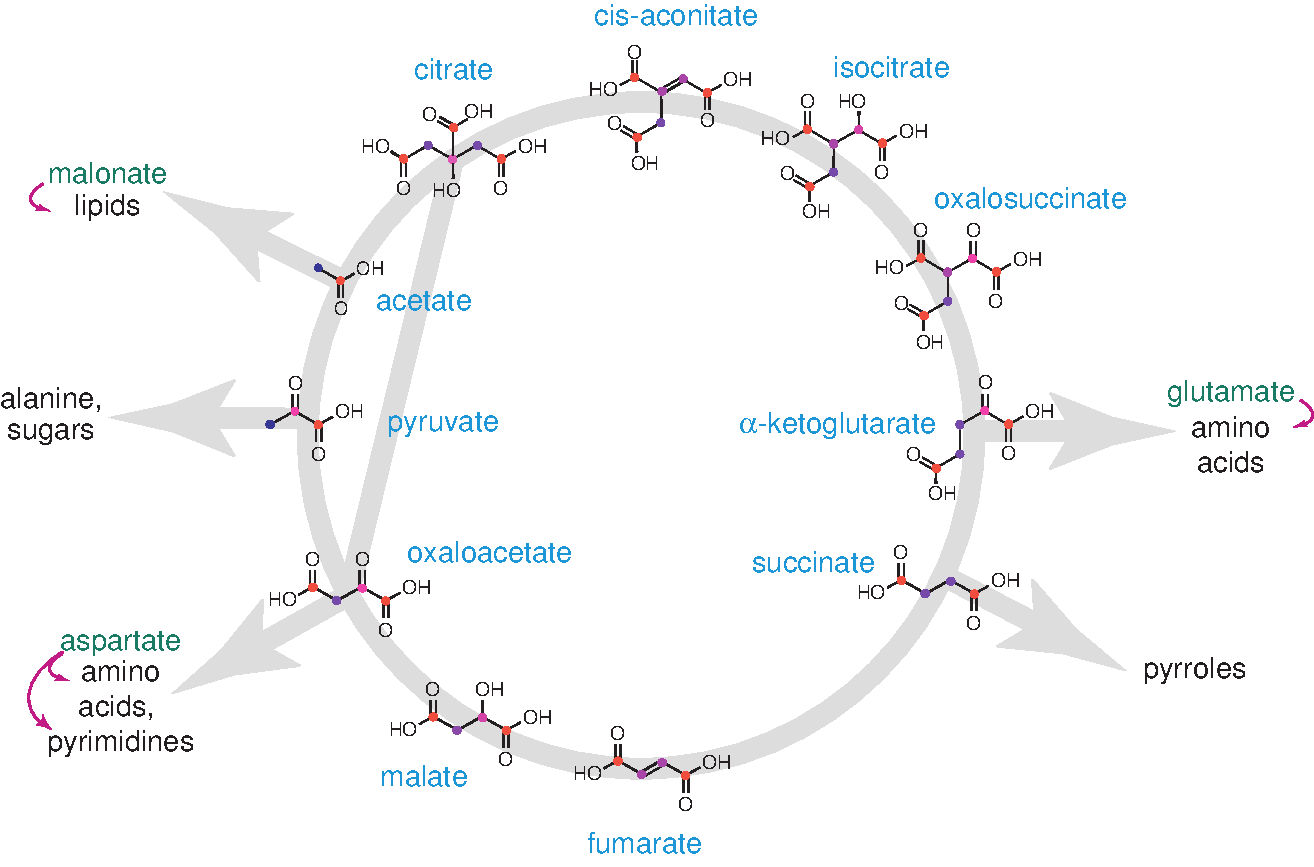
\includegraphics[width=0.7\columnwidth]{fig/rTCA-skeleton.pdf}
\end{center}
\caption[TCA cycle]{A depiction of the structure of the citric acid cycle and the products of the associated pathways for which it generates substrates. This figure is adapted from~\cite{Braakman2012a}.}
\label{fig:ctacyc}
\end{figure}

A situation analogous to the enzyme-substrate-product abstraction is formalized in a fundamental manner in type theory, category theory and the relationship between them (see \ref{sec:ctbackground}). That a distinction between object and morphism was perhaps conceptually fruitful was originally suggested in Russell and Whitehead's type theory as a means of circumventing the self-referential Russell's (also known as Barber's) paradox of set theory in which one can not determine internal to the language of set theory whether a set of all sets that contain themselves contains itself or not \cite{Bell2012}. In type theory a hierarchy is introduced that is analogous to the distinction fundamental to the definition of a category in category theory between objects (which are like substrates and products in terms of metabolic networks) and morphisms (which play the role of enzymes). In category theory, this distinction propagates up a hierarchy of higher-order functions where if we are in a category having a terminal, $1$, and exponential objects and we consider two objects $A$ and $B$ and morphisms between them, the collection of which is represented internal to a given category as a so-called exponential object $B^A$ or externally as the set $Hom(A,B)$ one of which might be $f \colon A \rightarrow B$ then the respective \emph{elements} of $A$, $B$ and $B^A$ can be related but not equivocated because they have different \emph{types}. From this perspective, while it is possible to \emph{evaluate} an element $f:B^A$ read ``an element $f$ of type $B^A$ given by $f \colon 1 \rightarrow B^A$'' at an element $a:A$ given by $a \colon 1 \rightarrow A$ to arrive at some element $b:B$ given by $b \colon 1 \rightarrow B$ it is not possible to likewise \emph{evaluate} an element $a:A$ at another element $a':A$ as this kind of statement is simply not able to be expressed within the confines of the language. If it were possible to do such a thing in some potentially more expressive meta-language, then we can imagine that in the reasoning described above we have restricted ourselves to a state in which we are completely unaware of this capacity.

The enzyme-substrate-product abstraction can be interpreted in terms of symmetric monoidal categories and depicted using corresponding string diagrams \cite{Co2010}. Any metabolic reaction such as one of the first steps in the tricarboxylic acid cycle depicted in \ref{fig:ctacyc} can be viewed as a morphism acting on tensored objects. The way this metaphor is constructed is to associate to a biochemical reaction such as
$$
\text{Oxaloacetate } + \text{Acetyl CoA} + H_2O \xrightarrow[]{\text{Citrate synthase}} \text{Citrate} + \text{CoA-SH},
$$
abstract labels
$$
s_1 + s_2 + s_3 \xrightarrow[]{m_1} p_1 + p_2.
$$
This can be done for any biochemical reaction and at any level of abstraction. For example we can do the same for the net reaction that occurs for each iteration of the TCA cycle as
$$
\text{Acetyl-CoA} + 3 \text{NAD}^+ + \text{Q} + \text{GDP} + P_i + 3 H_2O \xrightarrow[]{\text{TCA cycle}} \text{CoA-SH} + 3 \text{NADH} + 3H^+ + QH_2 + \text{GTP} + 2 CO_2,
$$
where we now have to abstract from a single enzyme to the composite action of all of the enzymes directly involved in the collection of reactions to which we give the name ``TCA cycle''. The abstract labels that may be associated with this biochemical transformation are
$$
s_1 + s_2 + s_2 + s_2 + s_3 + s_4 + s_5 + s_6 + s_6 + s_6 \xrightarrow[]{f} p_1 + p_2 + p_2 + p_2 + p_3 + p_3  + p_3 + p_4 + p_5 + p_6 + p_6.
$$
The general promiscuity of metabolic interactions in which enzymes recognize a collection of, for the most part very closely, related substrates suggests the representation of these biochemical reactions as tensor products of objects in a category. The intuition behind doing so lies in the fact that if there is a general class of substrates that can substitute for a given one, then instead of specifying a particular one, $s_1$, we should specify an entire set of them $S_1$. Then if there is another set, $S_2$ of substrates that can take the place of $s_2$, and the substrates upon which an enzyme acts is defined on $S_1 \times S_2$, then that enzyme can be said to act on any pair $(s_1,s_2)$ of substrates where $s_1 \in S_1$ and $s_2 \in S_2$. This case of viewing $S_1$ and $S_2$ as sets may come to be seen as being too restrictive in which case we would be forced to consider the abstract tensor product of two objects in a category $S_1 \otimes S_2$, which could then be specialized to cases other than those in which $S_1$ and $S_2$ are well-modelled as sets. For the simple example of the Citrate synthase catalyzed aldol condensation reaction described above, we arrive at a representation in terms of a morphism in a symmetric monoidal category
\begin{eqnarray*}
m_1 \colon S_1 \otimes S_2 \otimes S_3 &\longrightarrow& P_1 \otimes P_2\\
(s_1,s_2,s_3) &\longmapsto& (p_1,p_2)
\end{eqnarray*}
The adjective ``symmetric'' is appended to monoidal category based upon the assumption that the order of combination of substrates and production of products is unimportant and thus the factors of tensor products representing molecules may be permuted. The prototype example of such a monoidal category is the category of sets with cartesian product, but the formalism is not limited to this. We will proceed thinking in terms of this case as a useful mental crutch for grounding intuitions, but its limitations with respect to the capacity to recognize the full generality of the formalism at hand can be severe. Indeed, we will be forced to highlight at least one case where such intuition fails in order to express the functional closure concept in a non-trivial way.

\begin{figure}
\begin{center}
\noindent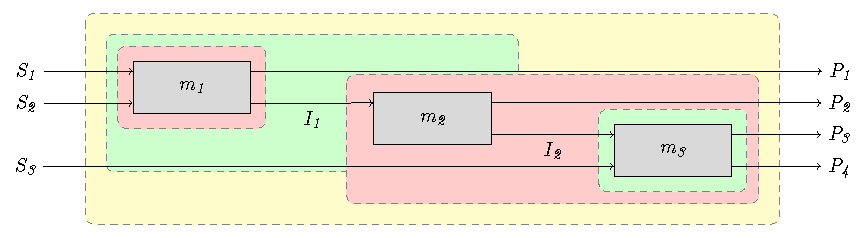
\includegraphics[width=0.9\columnwidth]{fig/blockdiagtop.pdf}
\end{center}
\caption[Abstraction of a metabolic network]{An abstraction of metabolic networks that can be interpreted in terms of symmetric monoidal categories and their associated string diagrams (see \ref{sec:ctbackground}).}
\label{fig:metabolicstringdiag}
\end{figure}

The metabolic network formalism interpreted in symmetric monoidal categories then applies to the case in which we string together metabolic processes. An example of this is presented in \ref{fig:metabolicstringdiag}. In this diagram, we have the following morphisms:
\begin{eqnarray*}
m_1 \colon S_1 \otimes S_2 &\longrightarrow& P_1 \otimes I_1,\\
m_2 \colon I_1 &\longrightarrow& P_2 \otimes I_2,\\
m_3 \colon I_2 \otimes S_3 &\longrightarrow& P_3 \otimes P_4.
\end{eqnarray*}
These morphisms can be composed as
$$
f \cong (m_1 \circ m_2) \circ m_3 \cong m_1 \circ (m_2 \circ m_3) \cong m_1 \circ m_2 \circ m_3,
$$
where further identifying $A \cong S_1 \otimes S_2 \otimes S_3$ and $B \cong P_1 \otimes P_2 \otimes P_3 \otimes P_4$ allows us to express any metabolic network represented in the form depicted in \ref{fig:metabolicstringdiag} regardless of the more or less complicated nature of intermediate interactions concisely as
$$
\xymatrix@1{
  A\ar[r]^-{f} & B.
  }
$$
In general we can consider any case of $f \colon \prod_i S_i \rightarrow \prod_j P_j$ as being denoted by $f \colon A \rightarrow B$ for $A \cong \prod_i S_i$ and $B \cong \prod_j P_j$. An element $a \colon A$ then represents a tuple $(s_1, s_2, \ldots, s_N)$ that expresses a state of metabolic input substrates and likewise for the metabolic products $b \colon B$ representing $(p_1, p_2, \ldots, p_M)$.

\begin{figure}
\begin{center}
\noindent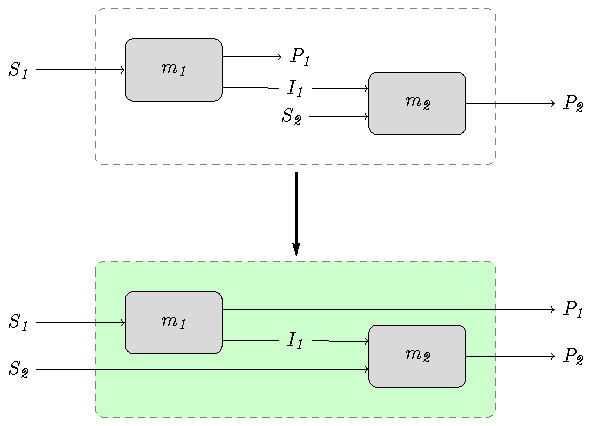
\includegraphics[width=0.5\columnwidth]{fig/blockassoclaw.pdf}
\end{center}
\caption[Graph rewriting metabolic networks]{A demonstration of a simple graph rewrite or reduction rule that can be applied to metabolic processes. This rule can be used in the reduction of a simple model of the citric acid cycle to an effective network.}
\label{fig:stringassoclaw}
\end{figure}

A graph rewrite rule can be derived from the associative composition law that is valid in symmetric monoidal categories in terms of string diagrams like that of \ref{fig:metabolicstringdiag}. In this case we have template metabolic processes given by
\begin{eqnarray*}
m_1 \colon S_1 &\longrightarrow& P_1 \otimes I_1,\\
m_2 \colon I_1 \otimes S_2 &\longrightarrow& P_2,
\end{eqnarray*}
shown in the top panel of \ref{fig:stringassoclaw}. Following the application of the rewrite rule presented in \ref{fig:stringassoclaw} we have the composite effective metabolic process
\begin{eqnarray*}
m_{1}m_{2} \equiv m_1 \circ m_2 \colon S_1 \otimes S_2 &\longrightarrow& P_1 \otimes P_2,
\end{eqnarray*}
where we note that the intermediate $I_1$ has been eliminated from both the inputs and outputs of the $m_1$ and $m_2$ processes.

This formalism has been previously applied, albeit not in the explicit context of symmetric monoidal categories, to reduce via associative composition the citric acid cycle to a smaller collection of effective reactions. The steps involved in this process are depicted in \ref{fig:ctacycred}. The fully reduced form of the citric acid cycle presented in \ref{fig:ctacycred}d will be used in what proceeds to provide a biological example with respect to which the additional molecular interactions that may be necessary in order to achieve functional closure may be defined.

\begin{figure}
\begin{center}
\noindent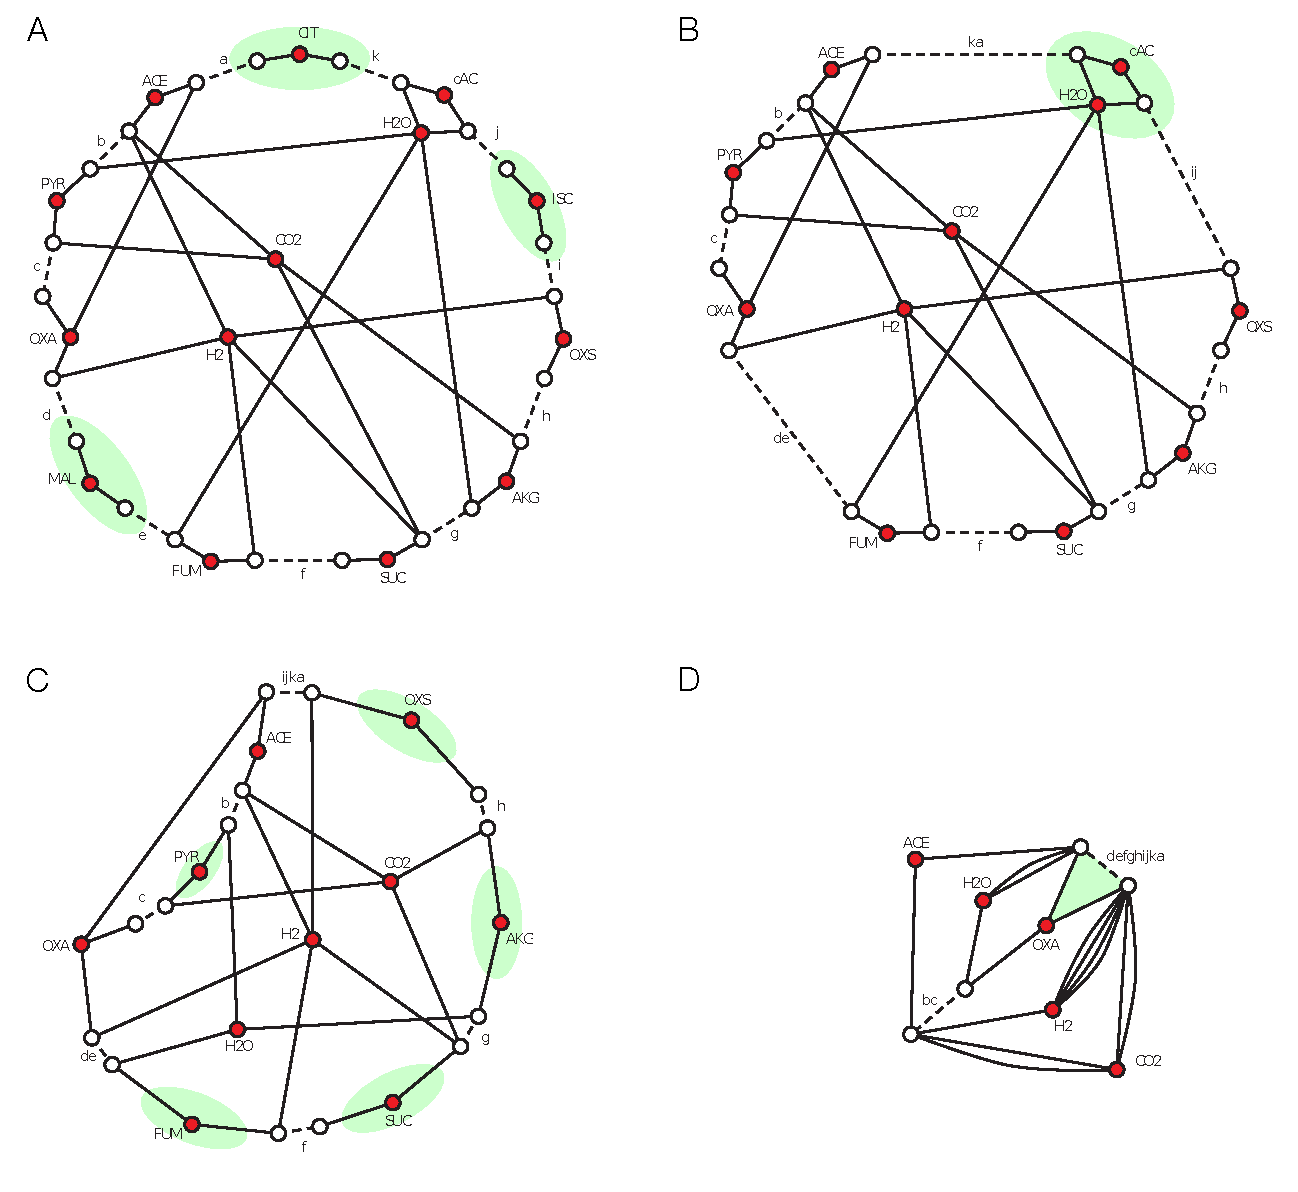
\includegraphics[width=0.9\columnwidth]{fig/rTCA-reduction.pdf}
\end{center}
\caption[TCA reduction]{A demonstration of the reduction of the biochemical reactions comprising the citric acid cycle according to the graph rewrite rule depicted in Figure~\ref{fig:stringassoclaw}. This figure is adapted from the citric acid cycle reduction process developed in~\cite{Braakman2012a}.}
\label{fig:ctacycred}
\end{figure}


\section{Functional closure}\label{sec:functionalclosure}

\subsection{Theoretical Background}

From the perspective described in
%\ref{sec:exampleformalmetabolicreaction},
\ref{sec:metabolismabstraction},
we can look at biochemical reaction networks as processes that compute outputs from inputs. If we are willing to abstract over intermediates, we can take what may appear to be an incredibly complicated reaction network and reduce it to its salient topological features. In doing this, regardless of whether it is justified or not from a scientific perspective, we make implicit use of the algebra of functions that can in principle be associated with a reaction network.

Category theory formalizes the algebra of functions \cite{Lane1998,Lawvere2003,Awodey2006}. Although category theory is independent of and even departs from some of the basic concepts of set theory, thinking about sets and functions between them is a good way to anchor intuition.  In order to understand category theory, it is necessary to recognize that there is some sense in which everything one knows intuitively about sets that requires reasoning explicitly about their elements, can be represented without ever directly referring to their elements in the colloquial sense, but rather by referring only to mappings between sets.

The definitions of a category and exponential object are provided here for reference because they are used directly. More detail is provided in \ref{sec:ctbackground} and the associated references. The versions of these standard definitions that follow are adapted from \cite{Planetmath}.

% \begin{figure}[!htbp]
% \centering
% \noindent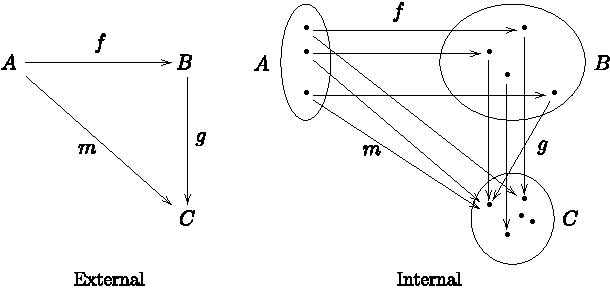
\includegraphics[width=0.8\columnwidth]{fig/intextdiag.pdf}
% \caption[Internal and external perspective of sets and mappings]{The internal and external perspective on sets, functions between them, and composition of those functions \cite{Lawvere2003}.}
% \label{fig:category}
% \end{figure}

\begin{definition}[category]
A \emph{category} $\mathcal{C}$ consists of:
\begin{enumerate}
\item a class $\operatorname{ob}(\mathcal{C})$ of objects (of $\mathcal{C}$)
\item for each ordered pair $(A,B)$ of objects of $\mathcal{C}$, a collection $\hom(A,B)$ of morphisms from the domain $A$ to the codomain $B$
\item a function $\circ:\hom(A,B)\times\hom(B,C)\to\hom(A,C)$ called composition.
\end{enumerate}
\end{definition}
Denote $\circ(f,g)$ by $g \circ f$ for morphisms $f,g$. The above must satisfy the following conditions: for objects $A,B,C,D$,

\textbf{A1}: $\hom(A,B) \cap \hom(C,D)=\emptyset$ whenever $(A,B)\neq (C,D)$, i.e. the intersection is non-trivial only when $A=C$ and $B=D$.

\textbf{A2}: (Associativity) if $f \in \hom(A,B)$, $g\in\hom(B,C)$ and $h\in\hom(C,D)$, $h\circ (g\circ f)=(h\circ g)\circ f$

\textbf{A3}: (Existence of an identity morphism) for each object $A$ there exists an identity morphism $ {}id_{A}\in\hom(A,A)$ such that for every $f\in\hom(A,B)$, $f\circ id_{A}=f$ and $ {}id_{A}\circ g=g$ for every $g \in \hom(B,A)$.

\begin{definition}[exponential object]
Let $A,B$ be objects in a category with finite products $\mathcal{C}$.  An object $E$ in $\mathcal{C}$ is called an \emph{exponential object} from $A$ to $B$ if it satisfies the following conditions:
\begin{itemize}
\item there is a morphism $f:E\times A\to B$, called an \emph{evaluation morphism}
\item for any morphism $g:C\times A\to B$, there is a unique morphism $h:C\to E$ such that $f\circ (h\times 1_A)=g$, where $h\times 1_A:C\times A\to E\times A$ is the product morphism of $h$ and the identity morphism on $A$.
\end{itemize}
Thus, the following diagram must commute where $h$ is uniquely determined by $g$
\[
\begin{tikzcd}[row sep=tiny,ampersand replacement=\&]
E \times A \arrow{dr}{f} \\
{} \& B \\
C \times A \arrow[dashed]{uu}{h \times 1_A} \arrow{ur}[swap]{g} \&
\end{tikzcd}
\]
\end{definition}

Any two exponential objects from $A$ to $B$ are isomorphic, hence the existence of an exponential object between two objects is a universal property.  We may write $B^A (\cong E$ above) \emph{the} exponential object from $A$ to $B$.
\vskip 1mm
For example, in the category of sets, $\textbf{Set}$, where products exist between pairs of objects (sets), the exponential from $A$ to $B$ is the set $B^A$, which is defined as the set of all functions from $A$ to $B$.

In mathematical logic, one finds yet another usage of terminology, which, at first glance, appears to be equivalent to the simple notions of sets and elements: these are types and elements or inhabitants of those types. It is possible to determine a mapping or dictionary from type theory to category theory and vice versa. This is exemplified by the relationship between what is referred to as the simply-typed $\lambda$-calculus and its counterpart in category theory referred to as the Cartesian closed category.

The simply-typed $\lambda$-calculus is made up of types, terms and equations as follows:
\begin{enumerate}
\item{Types:}
\begin{align*}
&\mbox{basic types: } A, B, \ldots\\
&\mbox{product types: } A \times B, \ldots\\
&\mbox{function types: } A \rightarrow B, \ldots
\end{align*}
\item{Terms:}
\begin{align*}
&\mbox{variables: } x, y, z, \ldots \colon A \mbox{ for each type } A,\\
&\mbox{constants: } a \colon A, b \colon B, \mbox{ for each type},\\
&\mbox{products: }\langle a, b \rangle \colon A \times B \mbox{ for } a:A \mbox{ and } b:B,\\
&\mbox{first projection: }\mbox{fst}(c) \colon A \mbox{ for } c \colon A \times B,\\
&\mbox{second projection: }\mbox{snd}(c) \colon A \mbox{ for } c \colon A \times B,\\
&\mbox{application: }ca \colon B \mbox{ for } c \colon A \rightarrow B \mbox{ and } a \colon A,\\
&\mbox{abstraction: }\lambda x. b \colon A \rightarrow B \mbox{ for } x \colon A \mbox{ and } b \colon B
\end{align*}
\item{Equations:}
\begin{align*}
            \mbox{fst}(\langle a, b \rangle) &= a\\
            \mbox{snd}(\langle a, b \rangle) &= b\\
            \langle \mbox{fst}(c), \mbox{snd}(c) \rangle &= c\\
            (\lambda x.b)a &= b[a/x]\\
            \lambda x.cx &= c, \mbox{ $x$ not in $c$ }\\
            \lambda x.b &= \lambda y.b [y/x], \mbox{ no $y$ in $b$ }
\end{align*}
\end{enumerate}

Depending upon the specific from of allowed types, terms, and equations, there are many different kinds of lambda calculi. Several of these have been related in a schematic known as the Barendregt lambda cube  \cite{Barendregt1985}, \ref{fig:lambdacube}. The bottom left corner $\lambda_{\rightarrow}$ corresponds to the simply-typed $\lambda$-calculus. Moving in any of the indicated directions along the edges of the cube is associated to a particular kind of generalization of the simply-typed $\lambda$-calculus: terms depending on types (up), types depending on types (into page), types depending on terms (right). The far corner of the cube corresponds to a language containing all three of these generalizations.

\begin{figure}[!htbp]
\centering
\noindent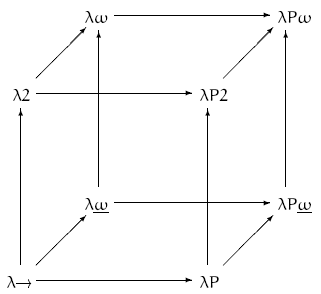
\includegraphics[width=0.5\columnwidth]{fig/lambda-cube.png}
\caption{The Barendregt lambda cube}
\label{fig:lambdacube}
\end{figure}

The simply-typed $\lambda$-calculus is essentially equivalent to a cartesian closed category (see \ref{sec:ctbackground}) in a sense that has been made precise. Both are languages in which it is possible to express transformations via functions between objects with operations that express pairing, projection, and application.

To any language $\mathcal{L}$ satisfying the defining equations of the simply-typed $\lambda$-calculus, a cartesian closed category of types $\mathcal{C}(\mathcal{L})$ is determined by the following identifications \cite{Awodey2000,Awodey2006}
\begin{enumerate}
\item{objects: } types
\item{morphisms: } terms $c \colon A \rightarrow B$ that are identified for $c \sim c'$ given by the equivalence relation determined by the defining equations of $\lambda$-calculus. Two equivalence classes of terms $[a], [b]$ may be identified $[a] = [b]$ if and only if the terms they represent are equivalent, which is to say that  $\mathcal{L} \vdash a = b$.
\item{identities: } $1_A = \lambda x.x$ where $x \colon A$
\item{morphism composition: } $c \circ b = \lambda x.c(bx)$
\end{enumerate}

If we refer to the set of basic types, terms, and equations as a \emph{theory}, $\mathcal{L}$, in the $\lambda$-calculus, then $\mathcal{C}(\mathcal{L})$ is the cartesian closed category presented by the generators (types and terms) and relations (equations) stated by the $\lambda$-calculus over $\mathcal{L}$. A model of such a theory $\mathcal{L}$ in the $\lambda$-calculus in a cartesian closed category $\mathcal{C}$ is given by an assignment of types and terms in $\mathcal{L}$ to objects and morhphisms in $\mathcal{C}$:
\begin{align*}
X \mbox{ basic type } &\leadsto \llbracket X \rrbracket\\
b \colon A \rightarrow B \mbox{ basic term } &\leadsto \llbracket b \rrbracket \colon \llbracket A \rrbracket \rightarrow \llbracket B \rrbracket
\end{align*}
which can be naturally extended to the other types and terms that are built upon these. Moreover the equations associated to the theory $\mathcal{L}$ are required to be satisfied so that:
\begin{align*}
\mathcal{L} \vdash [a]=[b] \colon A \rightarrow B \Longrightarrow \llbracket a \rrbracket = \llbracket b \rrbracket \colon \llbracket A \rrbracket \rightarrow \llbracket B \rrbracket
\end{align*}
This semantic association between a theory $\mathcal{L}$ in $\lambda$-calculus and models of such theories in cartesian closed categories is referred to as \emph{denotational semantics} for the $\lambda$-calculus \cite{Britain1980,Scott1980,Scott2000,J.Lambek177,Awodey2000,Awodey2006}.

\subsection{Functional closure as a potentially invariant property of evolvable systems}\label{sec:funclosinvarevo}

In this section, we give an example of the functional closure property. We describe this property in the setting of a cartesian closed category (see \ref{sec:ctbackground}). Cartesian closed categories provide mathematical semantics for the simply-typed $\lambda$-calculus \cite{Barendregt1985}. We will therefore sometimes refer to this setting as being \emph{typed}. This terminology is used to contrast the description in this section in terms of a cartesian closed category, which could be given equally well in terms of simply-typed $\lambda$-calculus, with that in the next section in terms of the untyped $\lambda$-calculus. The abstract components have been related to biological ones in \ref{sec:metabolismabstraction}. The biological phenomenon from which examples satisfying the functional closure condition are derived is metabolism regarded in the manner described in \ref{sec:metabolismabstraction} and as depicted in \ref{fig:metabolicstringdiag}. A metabolic mapping in an evolvable system $\mathcal{E}$ can be thought of as a morphism between two objects in $\mathcal{E}$, the latter now regarded as an abstract algebraic category:
\begin{align*}
f \colon A &\longrightarrow B\\
a &\longmapsto f(a)=b
\end{align*}

In category theory, we can imagine the abstract objects and morphisms as specializing to a particular type of algebraic structure and, thus, as a first approximation we can think of both objects as (cartesian product) sets, where $A$ represents a configuration of input substrates and $B$ likewise for metabolite products of metabolic transformations such as $f$. This abstraction of some aspects of an evolvable system could be further developed by substituting more highly structured objects than sets that meet intuitive and otherwise empirically suggested features of evolvable systems. We can consider all such \emph{metabolisms} together as the set of all the different morphisms between these objects referred to, if such an object exists at all, as the \emph{internal} exponential object $B^A$ \footnote{see \ref{sec:ctbackground} for the precise definition of exponetial object} or the \emph{external} hom-set $Mor_{\mathcal{E}}(A,B)$.

The finite chemical constitution of evolvable systems imposes constraints deriving from the requirement to maintain sufficient concentrations of the components that constitute it. As enzymes necessary for metabolism decay, they must be regenerated, from the metabolic products, or the system comprised of them will disintegrate. In addition, fluctuations in the substrates $A$ have to be corrected by the differential availability and performance of the overall metabolic morphism $f$. Hence, within the collection of morphisms from $B$ to $B^A$, at least one may be identified with the information required to \emph{regenerate} the enzymes necessary for core metabolic processes:
\begin{align*}
g \colon B &\longrightarrow B^A\\
b &\longmapsto g(b)=f
\end{align*}
This \emph{regeneration} system itself represented by $g \in B^{A^B}$ is also assumed to have a finite lifetime and thus requires a form of \emph{meta-regeneration} by some other system:
\begin{align*}
h \colon B^A & \longrightarrow B^{A^B}\\
f & \longmapsto h(f)=g.
\end{align*}
In the biological metaphor commonly associated to this abstract construction, this \emph{meta-regeneration} system is associated to the maintenance of some approximate structural invariance in the topology of the combined gene regulatory and metabolic interaction networks underlying an organism. In this light, this process may be associated to the DNA replication and reproduction process. In any case, the argument proliferating hierarchical levels of organization may, in principle, be continued \emph{ad infinitum} (i.e. the next step would be to ask for the origin of $h$ and to posit the existence of another higher-order morphism that takes $g$ as input and produces $h$, see \ref{fig:hom}B). Functional closure is considered to be achieved or satisfied if this process can be truncated at some level by identifying one of the higher-level functions as being able to be performed by one of the lower-level entities, such as $h \equiv b$.

If we follow this path considering only its algebraic properties, we see, in the absence of an ability to achieve closure precisely, the potential for generating an infinite hierarchy of functions of increasing order \ref{fig:speciesclosure}. The logical implications of admitting transformations of the kind that appear to achieve functional closure are not necessarily clear \emph{a priori}. From a logical perspective, it appears that functional closure requires one to allow a single element to have two different types, \ref{fig:hom}. This is certainly not allowed by the simply-typed $\lambda$-calculus.

\begin{figure}[!htbp]
\centering
\noindent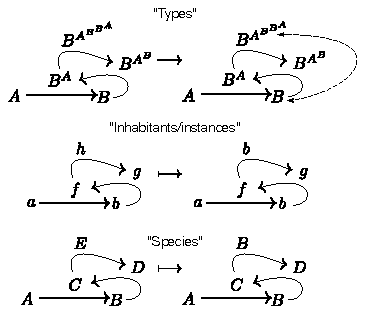
\includegraphics[width=0.5\columnwidth]{fig/speciesclosure.pdf}
\caption[Relationship of types, inhabitants, and species of reaction networks]{(left) A hierarchy of function types of increasing order, type inhabitants, and representation of those inhabitants as chemical species. (right) Imposition of functional closure by the arbitrary identification of inhabitants across types}
\label{fig:speciesclosure}
\end{figure}

From a biological perspective, systems of the form described may be able to avoid such an infinite regress by achieving a form of \emph{functional closure} in which, for example, we can materially identify a metabolic product $B$ with a replication function $h$ or perhaps even with the entire set of replication functions ${{{{B^A}^B}^B}^A}$. If we take the former case then we have introduced a problem that cannot be dealt with given the definition of a cartesian closed category alone because of the fundamental typing distinction therein between objects and morphisms. Although we might be able to associate an element or point of the object or type $B$ with $h \in {{{{B^A}^B}^B}^A}$, we confront a \emph{type error} if we attempt to express the fact that these are supposed to be somehow equivalent because $h \colon 1 \rightarrow B$ is of type $B$ while $h \colon B^A \rightarrow B^{A^B}$ is of type ${{{{B^A}^B}^B}^A}$. Thus we would attempt to state $h:B = h:{{{{B^A}^B}^B}^A}$, but this is impossible to do, at least naively, within a cartesian closed category associated to the simply-typed $\lambda$-calculus.  The type error arises due to the fact that equations are only allowed between elements (respectively paths) with the same type (respectively with the same domain and codomain) \ref{fig:hom}A. The other option is to avoid attempting to identify such elements and attempt to identify objects themselves. In this sense, we would attempt to express closure internally as $B \cong {{{{B^A}^B}^B}^A}$ or externally as $Mor_{\mathcal{E}}(1,B) \cong Mor_{\mathcal{E}}(B^A,B^{A^B})$. This approach could be considered to solve the typing issue in the category of sets since we could more explicitly state that $B \colon Set \cong {{{{B^A}^B}^B}^A} \colon Set$ or more generally for any category $B \colon Ob(\mathcal{E}) \cong {{{{B^A}^B}^B}^A} \colon Ob(\mathcal{E})$. However, we have now implied something stronger and less intuitive about the biological meaning of functional closure by stating that the set of metabolites is somehow isomorphic to the set of \emph{all possible} replication morphisms. Moreover, if such a relationship were to be satisfied, it could only be satisfied by the most trivial case in the category of sets $A = \{*\} = B$ so that $|B|=1=|{{{{B^A}^B}^B}^A}|$.

We have not yet attempted to make explicit how it might be possible to perform the identification between an element of type $B$ and another of type ${{{{B^A}^B}^B}^A}$ as expressed in \ref{fig:hom}C. The original argument describing functional closure in a sense settles for stating something weaker than what we have already suggested is impossible to do directly within the cartesian closed categories associated to the simply-typed $\lambda$-calculus (i.e. to state for some $h$, $h:B = h:{{{{B^A}^B}^B}^A}$). The most important feature of this argument is the concept of an evaluation map (see \ref{sec:ctbackground}), which is intrinsic to the definition of exponential objects and thus evaluation maps exist in certain categories, like the primary example of the category of $\mathbf{Sets}$ we have considered thus far, having such exponential objects. Given a category with products and exponentials, the evaluation map can be curried (i.e. in this case a function of two variables that returns a value can be converted to a function of one variable that returns a function) in the following manner
\begin{prooftree}
        \AxiomC{$B^{A} \times A \xrightarrow[]{ev} B$}
        \UnaryInfC{$A \xrightarrow[]{\hat{ev}} B^{B^A}$}
\end{prooftree}
where the maps $\hat{ev}$ are defined pointwise as
\begin{align*}
\hat{ev}(a) \equiv ev_a \colon B^A &\longrightarrow B,\\
f &\longmapsto ev(f,a) = f(a).
\end{align*}
This construction can be applied analogously at the next level regarding the evaluation of functions of the type $B^{A^B}$, by applying them to arguments of type $B$, to functions of the type $B^A$. The currying of the evaluation map is given by
\begin{prooftree}
        \AxiomC{$B^{A^B} \times B \xrightarrow[]{ev} B^A$}
        \UnaryInfC{$B \xrightarrow[]{\hat{ev}} B^{A^{B^{A^B}}}$}
\end{prooftree}
where the maps $\hat{ev}$ are defined pointwise as
\begin{align*}
\hat{ev}(b) \equiv ev_b \colon B^{A^B} &\longrightarrow B^A,\\
g &\longmapsto ev(g,b) = g(b).
\end{align*}
Although functional closure may also occur at the first level associated to $ev_a$, we consider its occurence at the next level involving $ev_b$ to maintain the intuitive property that the metabolic substrate configuration represented by $A$ also represents material being extracted from the environment while, biologically, functional closure is assumed to be achieved by the combination of the metabolic network (represented by $f$) and the regulatory apparatus (represented by $g$ and $h$) layered on top of it with $A$ serving as the necessary environmental input to such a non-equilibrium system defined by $(f,g,h)$.

Consider the preimages of the evaluation morphisms
\begin{align*}
\hat{ev}^{*}(b) \equiv ev^{*}_b \colon B^A &\longrightarrow B^{A^B},\\
f &\longmapsto g |g(b)=f.
\end{align*}
If, in this case, the evaluation morphism can be shown to have an inverse
% (i.e. $\hat{ev}^{*} \circ \hat{ev} = 1_A$ and $\hat{ev} \circ \hat{ev}^{*}= 1_{B^{B^A}}$)
(i.e. $\hat{ev}^{*} \circ \hat{ev} = 1_B$ and $\hat{ev} \circ \hat{ev}^{*}= 1_{{{{{B^A}^B}^A}^B} }$)
for some potentially restricted domain of definition of $\hat{ev}$ then the inverse morphism can also be defined pointwise as
\begin{align*}
\hat{ev}^{-1}(b) \equiv ev^{-1}_b \colon B^A &\longrightarrow B^{A^B},\\
f &\longmapsto g | g(b) = f.
\end{align*}
In this sense, if there is a unique $g$ satisfying $g(b)=f$ for each combination of $b$ and $f$ in the potentially restricted domains of definition then $b$ and $f$ can be viewed as determining $g$ among other possibilities. This is a weaker statement supported by the preceding argument as compared to the stronger version that attempts to identify $b:B = h:{{{{B^A}^B}^B}^A}$. If determination among extant possibilities is considered to be sufficient for functional closure, then this would allow for the truncation of what was otherwise demonstrated to lead to infinite regress as a result of the continued necessity of positing the existence of an $h:{{{{B^A}^B}^B}^A}$ to answer the question of the origin of some $g$, and to continue to do similarly for higher levels. On the other hand, the stronger form of functional closure can be expressed in a more expressive language that does not enforce typing discipline in the same was as the simply-typed $\lambda$-calculus and its associated cartesian closed category.

\begin{figure}
\begin{center}
\noindent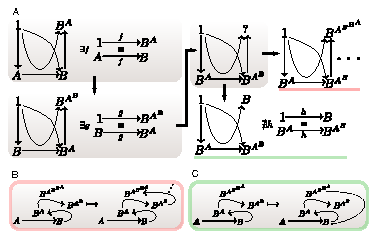
\includegraphics[width=0.75\columnwidth]{fig/mrcatclosure.pdf}
\end{center}
\caption[Functional closure in a Cartesion closed category]{Attempting a depiction of functional closure in a cartesian closed category. (A) The top-left panel shows the identification of morphisms with domain $A$ and codomain $B$ with elements of the exponential object $B^A$. The bottom-left panel shows the analogous relationship between morphisms with domain $B$ and codomain $B^A$ and the exponential object $B^{A^B}$. On the right, two alternatives are shown in the last step. Either one can (B) continue on the path leading to infinite regress or (C) take the path leading to closure at some \emph{level}. The case depicted here suggests closure at the third level via identification of some $b:B$ with some $h:{{{{B^A}^B}^B}^A}$}
\label{fig:hom}
\end{figure}

\subsection{Functional closure expressed in a type-free setting}
This argument describing functional closure so far suggests constraints by which we may be able to \emph{determine} some $h$ via $b$ (and also $f$), but so long as the ultimate goal is to state that for some $b$, $b:B = h:{{{{B^A}^B}^B}^A}$, it cannot be done in an obvious way. This is a result of the typing discipline inherent to the simply-typed description used thus far. It is ultimately possible to express the stronger form of the functional closure property in category theoretic terms, but additional conditions are required on top of those of cartesian closure. We first re-consider the expression of functional closure in terms of the type-free or untyped $\lambda$-calculus, \cite{Barendregt1985}, before returning to the so-called categorical semantics that enable the re-expression of this stronger form of functional closure in category theoretic terms.

If we reconsider the discussion in the previous section without regard for any typing discipline, we can summarize the proliferation of levels of organization up through the first three discussed in the following system of equations~\cite{Mossio2009}
\begin{align*}
f(a)&=b,\\
g(b)&=f,\\
h(f)&=g.
\end{align*}
It is trivial to express the functional closure property so long as we are able to disregard any typing discipline by identifying $h$ with $b$. In this case we can express functional closure as
\begin{align*}
f(a)&=b,\\
g(b)&=f,\\
b(f)&=g.
\end{align*}
If we collapse these terms we arrive at the expression
\begin{equation}\label{eq:frec}
f = gb = [bf]b = [[fa]f](fa).
\end{equation}
We can write the right hand side directly in $\lambda$-calculus syntax as the lambda term $M$
$$
M = \lambda x.((xa)x)(xa).
$$
Given that \ref{eq:frec} states that $f$ is a fixed point of the term $M$, we can use the fixed point combinator $\mathbf{Y} = \lambda f.(\lambda x. f (x x))(\lambda x. f (x x))$ to write $f$ in terms of $\mathbf{Y}$ and $M$ as
$$
f = \mathbf{Y}M.
$$

It is clear that in the typed setting this is not possible. This is a result of the typing errors described in \ref{sec:funclosinvarevo} that occur in this case and it is related to the fact that the fixed-point combinators like $\mathbf{Y}$, of which there are an infinite number in the type-free $\lambda$-calculus, are known not to exist in the simply-typed $\lambda$-calculus. In the typed setting we worked within the language of a cartesian closed category, which, as mentioned, provides mathematical semantics for the simply-typed $\lambda$-calculus. Therefore, we may ask which language has sufficient expressive power to be able to state the functional closure property. We have just noted that the functional closure property can be directly expressed if we remove the typing constraint. This involves passing from the simply-typed to the type-free $\lambda$-calculus. We will explain the syntax of the type-free $\lambda$-calculus and then, by analogy to the fact that cartesian closed categories provide semantics for the simply-typed $\lambda$-calculus, we will consider which mathematical structure is capable of providing mathematical semantics for the type-free $\lambda$-calculus.

In \ref{sec:ctbackground}, we provide a description of the syntax of the simply-typed $\lambda$-calculus and its semantics in terms of cartesian closed categories that was used in attempting to develop a model of functional closure in terms of a cartesian closed category. We have suggested that in order to be able to obtain a strong notion of equivalence between an object and a morphism, we need a language with at least some of the expressive capability of the type-free $\lambda$-calculus. We will therefore develop the analogous constructions of syntax and corresponding categorical semantics for the type-free $\lambda$-calculus.

\subsubsection{The type-free lambda-calculus and its categorical semantics}
The type-free $\lambda$-calculus can be seen as a special case of the simply-typed $\lambda$-calculus in which the set of basic types is restricted to contain only a single one. With the typing constraint imposed by having multiple types removed, it should be possible to perform self-application as in the term $\lambda x. xx$. If the second occurence of $x$ in this term has type $D$ and the whole term $xx$ has type $D$ then the first occurrence of $x$ in the term $xx$ must be construable as having type $[D \rightarrow D]$. A presentation of the type-free theory, $\mathbb{T}$, can then be given in a manner analogous to that of the simply-typed $\lambda$-calculus~\cite{Awodey2000}:
\begin{enumerate}
\item{Types:}
\begin{align*}
&\mbox{one basic type: } D\\
\end{align*}
\item{Terms:}
\begin{align*}
&\mbox{variables: } x,y,z, \ldots \colon D\\
&\mbox{constants: } i \colon [D \rightarrow D] \rightarrow D,\,\, r \colon D \rightarrow [D \rightarrow D]\\
\end{align*}
\item{Equations:}
\begin{align*}
            \lambda x. ri(x) &= \lambda x.x\\
            \lambda x. ir(x) &= \lambda x.x
\end{align*}
\end{enumerate}
On this basis, we are led to the requirement that
$$
[D \rightarrow D] \cong D,
$$
which is a particular instantiation of a more general phenomenon referred to as a recursive domain equation. The process by which $[D \rightarrow D]$ is formed in the first place is via the internal Hom bifunctor $F \equiv [-,-] \colon \mathcal{C}^{op} \times \mathcal{C} \rightarrow \mathcal{C}$ on a category $\mathcal{C}$, which thereby restricts consideration for the purpose of finding denotational semantics for the type-free $\lambda$-calculus to categories $\mathcal{C}$ that are closed since this is a necessary condition for it to posses the necessary structure to define the internal Hom bifunctor. In this light, the solution $D$ to the equation $[D,D] \cong D$ is a fixed point $F(D,D) \cong D$ of the internal Hom bifunctor on some category $\mathcal{C}$.

Given these restrictions, it is obvious that it will not be sufficient in the search for non-trivial models of the type-free theory of the $\lambda$-calculus to restrict consideration to the category $\mathbf{Sets}$ because in such a category $F$ has a fixed point $D$ only when $D$ is the one element set: $D = \{*\}$. However, $\mathbb{T}$ does not necessarily prove $\lambda y.ir(y)=\lambda y.y$, which would be true for $D = \{*\}$. Because something provable in $\mathbf{Sets}$ is not necessarily provable in the type-free $\lambda$-calculus there is no sense in which semantics in the category $\mathbf{Sets}$ could be complete with respect to the type-free $\lambda$-calculus.

We will very briefly recapitulate a solution to this problem and refer to other sources for caveats and details~\cite{Barendregt1985,Smyth1982,Freyd1990,Abramsky1995,Cattani2007}. Here we follow \cite{Hindley2006}. Dana Scott introduced \emph{domains}, which can be viewed as \emph{continuous lattices} (this construction appears with minor modifications with respect to the purpose of the present exposition in terms of various other closely related kinds of objects and their associated categories such as complete partial orders and complete lattices among others). A continuous lattice is a complete lattice $D$ such that
$$
\forall d \in D, d = \bigvee \left\{ \bigwedge U \mid d \in U,\; U \mbox{ Scott-open},\; U \subseteq D \right\}
$$
where \emph{Scott-open} refers to a subset $U$ of a domain $D$ that is upward closed in the sense that if $\bigvee \Delta \in U$ for a directed subset $\Delta \subseteq D$ then $U \cap \Delta \neq \emptyset$ and Scott-continuous functions are required to be monotonic and preserve least upper bounds of directed subsets of their domains. These continuous lattices can be equivalently characterized in topological terms as $T_0$-spaces in which every continuous function $f \colon P \rightarrow D$ from a subspace $P \subseteq S$ can be extended to a Scott-continuous function $\hat{f} \colon S \rightarrow D$.

Domains of this form taken as objects and Scott-continuous functions between them taken as morphisms form cartesian closed categories where the internal-hom (i.e. exponential) objects are not sets, but rather complete lattices of Scott-continuous functions. Since these form a cartesian closed category they could be used as described above to provide semantics for the simply-typed $\lambda$-calculus. However, categories of domains can also be constructed that have reflexive objects, $D_\infty$, which solve the recursive domain equation $F(D_{\infty},D_{\infty})=D_{\infty}$ that arises naturally as described above in the analysis of the type-free $\lambda$-calculus since, there, objects serve both as arguments and as functions that can be applied to such arguments.

The way in which such solutions $D_\infty$ are constructed is via a generalization of the least fixed-point of a continuous function. A continous function $f \colon D \rightarrow D$ may have fixed-points $x$ such that $f(x)=x$. The least fixed-point for such a continuous function $f$ is then given by
$$
fix(f) = \bigvee_{n \in \omega} f^n(\bot)
$$
Now, we would like to extend this notion to the internal-hom bifunctor $F \equiv [-,-] \colon \mathcal{C}^{op} \times \mathcal{C} \rightarrow \mathcal{C}$ for $\mathcal{C}$ a category of continuous lattices and Scott-continuous functions. Given domains $D$ and $E$ as objects in such a category, we can define an \emph{embedding-projection pair} from $D$ to $E$ as a pair of Scott-continuous functions $i \colon D \rightarrow E$ and $r \colon E \rightarrow D$ such that $r \circ i = id_D$ and $i \circ r \leq id_E$ where the relation of order on functions is given pointwise. Reflexive domains are given by inverse limits (or projective limits, which are specializations of limits, as opposed to colimits, in category theory) of sequences of projections $r_n$ given by:
\begin{align*}
&D_0 = \mbox{ some object, $D$, in } \mathcal{C},\\
&D_1 = [D_0 \rightarrow D_0],\\
&D_{n+1} = [D_n \rightarrow D_n],\\
&(r_n \colon D_{n+1} \rightarrow D_n)_{n \in \omega}.
\end{align*}
The fact that a suitable choice for the initial embedding-projection pair $\langle i_0, r_0 \rangle$ ultimately requires that the limit of the above sequence of projections coincide with the colimit of the sequence of embeddings
$$
(i_n \colon D_{n} \rightarrow D_{n+1})_{n \in \omega}.
$$
It is eventually possible to obtain
$$
\lim_{\leftarrow} (D_n, r_n) \cong D_\infty \cong \lim_{\rightarrow} (D_n, i_n).
$$
and this particular construction of $D_{\infty}$ provides a fixed-point $\text{FIX}(F)$ so that $F(D_{\infty},D_{\infty}) = D_{\infty}$ solves the given recursive domain equation associated to the untyped $\lambda$-calculus. This allows us to interpret the terms of the untyped $\lambda$-calculus as being the objects and morphisms $D_{\infty}$ and $[D_{\infty},D_{\infty}]$ respectively, which are now seen to be one and the same since $D_{\infty} \cong D_{\infty}^{D_{\infty}}$.



\section{Discussion}
\subsection{Categorical semantics for type theory, more generally}
We have presented two particular cases of a more general paradigm referred to as categorical semantics (for logic or type theory). In a slightly more general situation we can imagine that a \emph{basic language} $\mathcal{L}$ consists of basic types and basic terms with type assignments \cite{Awodey2000}. A (type) \emph{theory} $\mathbb{T}$ consists of a set of basic type symbols, a set of basic terms, typed over the basic types, and a set of equations between terms in the language $\mathcal{L}[\mathbb{T}]$ of all terms over the basic language of basic types and terms.

A \emph{model} $\mathcal{M}$ of a theory $\mathbb{T}$ in a category $\mathcal{C}$ can be viewed as a functor $\mathcal{M} \colon \mathbb{T} \rightarrow \mathcal{C}$ that provides an interpretation of the types $\tau$ and terms $N(x) \colon \tau$ of $\mathcal{L}[\mathbb{T}]$ as objects $X$ and arrows $\llbracket N(x) \rrbracket \colon X \rightarrow \llbracket \tau \rrbracket$ in $\mathcal{C}$ such that the equations defining $\mathbb{T}$ between terms of $\mathcal{L}[\mathbb{T}]$ are satisfied by their interpretations in terms of \emph{commutative diagrams} (which define equations between paths) in $\mathcal{C}$. A model is said to be \emph{standard} if $\mathcal{C}$ is cartesian closed and the function types $\sigma \rightarrow \tau$ are always interpreted as exponential objects meaning that $\llbracket \sigma \rightarrow \tau \rrbracket = \llbracket \tau \rrbracket ^ {\llbracket \sigma \rrbracket}$.

A system of \emph{semantics} $\mathcal{S}$ for a type theory then consists of a class of models $\mathcal{M} \colon \mathbb{T} \rightarrow \mathcal{C}$ for each theory $\mathbb{T}$ in possibly different categories $\mathcal{C}$. $\mathcal{C}$-valued semantics refer to the collection of models that take values in a particular category $\mathcal{C}$.

A system of semantics $\mathcal{S}$ is said to be complete if the deductive calculus for syntactic equivalence is sound and complete with respect to $\mathcal{S}$. This means that for every theory $\mathbb{T}$ and any terms $M, N \in \mathcal{L}[\mathbb{T}]$, $\llbracket M \rrbracket_{\mathcal{M}} = \llbracket N \rrbracket_{\mathcal{M}}$ for every model $\mathcal{M} \in \mathcal{S}$ if and only if $\mathbb{T} \vdash M = N$.

\subsection{The typed-type-free spectrum}
Although we have presented the type-free and the simply-typed theories of $\lambda$-calculus as if the former is particular and the latter general, there is a sense in which we have observed two extreme points on a spectrum in which precisely the opposite may be the case \cite{Scott1980,Barendregt1985}. Dana Scott suggested the relationship in which type-free or unityped is a specific case of the simply-typed theory in \emph{Relating theories of the $\lambda$-calculus} \cite{Scott1980}. Barendregt challenges this point of view in his classic book on $\lambda$-calculus (see page 87) \cite{Barendregt1985}. The sense in which the simply-typed theory is more general is that models of the type-free $\lambda$-calculus \emph{come from} cartesian closed categories with reflexive objects, wherein a single reflexive object can serve as a model of the type-free $\lambda$-calculus. Moreover, as we have described, the cartesian closed category itself with potentially many objects representing the simple types corresponds to the simply-typed $\lambda$-calculus. So from this point of view it appears that the type-free $\lambda$-calculus is a special case of the simply-typed wherein we restrict ourselves to one special type of object: a reflexive domain.

On the other hand the expressive power of these two languages suggests the opposite point of view. The simply-typed $\lambda$-calculus can represent only a proper subset of recursive functions whereas the type-free $\lambda$-calculus is capable of expressing any given recursive function. Of course, this additional expressive power comes with the potentially undesirable property of being able to express incomputable functions whereas it may be undesirable to do this.

In either case it is clear that the conceptual space between the simply-typed and the untyped $\lambda$-calculi may contain a more desirable system in which linguistic expressive power can be elevated beyond that of the simply-typed case without incorporating the ability to accidentally or intentionally express constructs that aren't computable. Indeed much research has been performed on such languages with exceptionally important consequences for the future of computation \cite{Coquand1988,Frade2009}. We expect that incorporating ideas from modern type theories will enable substantial refinement of the expression of the functional closure property that appears to be essential to the existence of evolvable systems and this may increase the degree to which theoretical evolutionary biology and programming language theory interact.

\section{Classifying logics with respect to evolutionary processes over their terms}

Fontana and Buss developed a computer simulation whereby a Moran process was imposed upon $\lambda$ terms in the type-free $\lambda$-calculus \cite{Fontana1994,Fontana1996}. This was defined by generating a random population of terms and then simulating a process whereby pairs of randomly chosen terms were sampled, composed and replaced into the population along with the result of composition. A generation was completed by choosing a random individual for elimination; thereby satisfying the basic defining features of Moran processes \cite{Moran1958}. Because this simulation was performed using the type-free $\lambda$-calculus the population fixated on a collection of trivial identity functions $f = \lambda x. x$ since these trivially satisfy the relation $f(f) = f$ and are thus self-replicating terms.

Fontana and Buss referred to the latter system of identity functions as minimal chemistry zero, $MC0$, which is equivalent to achieving functional closure at the lowest level possible. They then proceeded to identify higher-order forms of functional closure by prohibiting the existence of such identity functions and observing the new equilibrium of the Moran process defining the collection of terms remaining in this case as $MC1$ and so on.

In light of the relationship between the expressions of functional closure or approximations thereof described in \ref{sec:functionalclosure}, this suggests that any logic such as the untyped or simply-typed flavors of $\lambda$-calculus can be considered as a model for a chemical system relative to the dynamics of a stochastic process such as the Moran process over its terms. As a result of the categorical semantics that may be associated to any such logic, and that any category can be associated to an underlying graph, it is possible to imagine a framework for exploring the space of population processes on logics. This involves positing the types terms and relations definitive of a particular logic, determining the categorical semantics of that logic, mapping the associated category to its underlying graph, considering a population process over that graph, finding the subgraph onto which that process fixates, embedding it as a subcategory within the categorical semantics of the originally defined logic and finally comparing the resulting categories, or equivalently logics, that result.

The ultimate goal of such a project would be to classify the different kinds of relationships between the initially defined logic and the \emph{stationary sublogic} of the process defined by allowing for arbitrary composition of terms within the confines of that logic. This may enable the identification of classes of logics capable of achieving functional closure at different levels of organization.

\section{Background}\label{sec:ctbackground}
\subsection{Categories}
Some of the mathematical definitions in this section constitute ``textbook'' material taken directly from \cite{Planetmath}. It is included here merely as a helpful reference to avoid requiring immediate consultation of other sources. This material is available, for example, in \cite{Lane1998,Lawvere2003,Awodey2006}.

An intuitive picture to which one can anchor intuition when thinking in category theoretic terms is presented in \ref{fig:intextdiag}. In category theory, one can always consider the duality between the intrinsic structure of \emph{objects} and the manner in which that intrinsic structure can be expressed externally in terms of patterns of constraints placed upon the relationships between \emph{morphisms} among objects.

\begin{figure}
\begin{center}
\noindent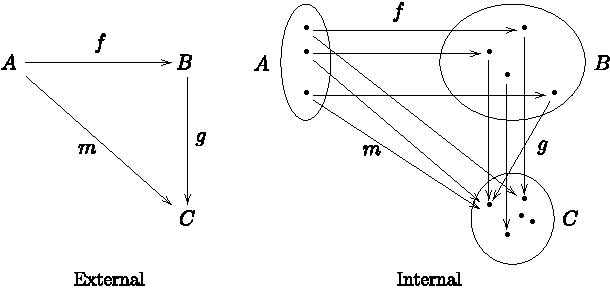
\includegraphics[width=0.8\columnwidth]{fig/intextdiag.pdf}
\end{center}
\caption[Function composition in an algebraic category]{In the external diagram on the left one simply considers \emph{objects} such as $A$,$B$, and $C$ and morphisms between them $f$, $g$, and $m$. The internal perspective, which in this case is specific to the category of $\mathbf{Sets}$, demonstrates the particular manner in which the equation $g \circ f = m$ may be satisfied in terms of the internal structure of the objects $A$, $B$, and $C$. Of course, in this case there are many other ways of satisfying the given equation; however, there are also questions that can be answered about the relationship between $A$, $B$, and $C$ given either $g \circ f = m$ or $g \circ f \neq m$ without necessarily knowing the particular manner in which either equation is satisfied by the relationships among the internal structures of the objects involved.}
\label{fig:intextdiag}
\end{figure}

A \emph{category} $\mathcal{C}$ consists of:
\begin{enumerate}
\item a class $\operatorname{ob}(\mathcal{C})$ of objects (of $\mathcal{C}$)
\item for each ordered pair $(A,B)$ of objects of $\mathcal{C}$, a collection (such as
 a set) $\hom(A,B)$ of morphisms from the domain $A$ to the codomain $B$
\item a function $\circ:\hom(A,B)\times\hom(B,C)\to\hom(A,C)$ called composition.
\end{enumerate}

Denote $\circ(f,g)$ by $g \circ f$ for morphisms $f,g$. The above must satisfy the following conditions: for objects $A,B,C,D$,

\textbf{A1}: $\hom(A,B) \cap \hom(C,D)=\emptyset$ whenever $(A,B)\neq (C,D)$, i.e. the intersection is non-trivial only when $A=C$ and $B=D$.

\textbf{A2}: (Associativity) if $f \in \hom(A,B)$, $g\in\hom(B,C)$ and $h\in\hom(C,D)$, $h\circ (g\circ f)=(h\circ g)\circ f$

\textbf{A3}: (Existence of an identity morphism) for each object $A$ there exists an identity morphism $ {}id_{A}\in\hom(A,A)$ such that for every $f\in\hom(A,B)$, $f\circ id_{A}=f$ and $ {}id_{A}\circ g=g$ for every $g \in \hom(B,A)$.

Some examples of categories:
\begin{itemize}
\item \textbf{0} is the empty category with no objects or morphisms, \textbf{1} is the category with one object and one (identity) morphism.
\item \textbf{Set} is the category of all small sets with morphisms being set functions
\item \textbf{Top} is the category of all small topological spaces with morphisms continuous functions
\item \textbf{Grp} is the category of all small groups whose morphisms are group homomorphisms
\end{itemize}

\textbf{Remark}.  If $\hom(A,B)$ in the second condition above is not required to be a set (but a class), we usually call $\mathcal{C}$ a \emph{large category}.

\subsubsection{Initial and terminal objects}
An {\em initial object} in a category $\mathcal{C}$ is an object $A$ in $\mathcal{C}$ such that, for every object $X$ in $\mathcal{C}$, there is exactly one morphism $A \longrightarrow X$. A {\em terminal object} in a category $\mathcal{C}$ is an object $B$ in $\mathcal{C}$ such that, for every object $X$ in $\mathcal{C}$, there is exactly one morphism $X \longrightarrow B$. A {\em zero object} in a category $\mathcal{C}$ is an object $0$ that is both an initial object and a terminal object. All initial objects (respectively, terminal objects, and zero objects), if they exist, are isomorphic in $\mathcal{C}$.

\subsubsection{Functors}
Given two categories $\mathcal{C}$ and $\mathcal{D}$, a covariant\ {\em functor} $T:\mathcal{C}\to\mathcal{D}$ consists of an assignment for each object $X$ of $\mathcal{C}$ an object $T(X)$ of $\mathcal{D}$ (i.e. a ``function'' $T:{\rm Ob}(\mathcal{C})\to{\rm Ob}(\mathcal{D})$) together with an assignment for every morphism $f\in{\rm Hom}_{\mathcal{C}}(A,B)$, to a morphism $T(f)\in{\rm Hom}_{\mathcal{D}}(T(A),T(B))$, such that:
\begin{itemize}
\item $T(1_A) = 1_{T(A)}$ where $1_X$ denotes the identity morphism on the object $X$ (in the respective category).
\item $T(g \circ f) = T(g)\circ T(f)$, whenever the composition $g\circ f$ is defined.
\end{itemize}

A contravariant functor $T :\mathcal{C}\to\mathcal{D}$ is just a covariant functor $T:\mathcal{C}^{\rm op}\to\mathcal{D}$ from the opposite category.  In other words, the assignment reverses the direction of maps.  If $f\in{\rm Hom}_{\mathcal{C}}(A,B)$, then $T(f)\in{\rm Hom}_{\mathcal{D}}(T(B),T(A))$ and $T(g\circ f) = T(f)\circ T(g)$ whenever the composition is defined (the domain of $g$ is the same as the codomain of $f$).

Given a category $\mathcal{C}$ and an object $X$ we always have the functor $T : \mathcal{C}\to{\bf Sets}$ to the category of sets defined on objects by $T(A) = {\rm Hom}(X, A)$.  If $f : A \to B$ is a morphism of $\mathcal{C}$, then we define $T(f) : {\rm Hom}(X,A)\to {\rm Hom}(X,B)$ by $g\mapsto f\circ g$.  This is a covariant functor, denoted by ${\rm Hom}(X,-)$.

Similarly, one can define a contravariant functor ${\rm Hom}(-,X) :\mathcal{C}\to{\bf Sets}$.

\subsubsection{Natural transformations}
Let $\mathcal{C}$ and $\mathcal{D}$ be categories, and let
$S,T:\mathcal{C}\to\mathcal{D}$ be covariant functors. Then suppose
that for every object $A$ in $\mathcal{C}$ one has a morphism
$\eta_A :  S(A) \to T(A) $ in $\mathcal{D}$ such that for every morphism
$\alpha: A \to B$ in $\mathcal{C}$ the following
$$
\xymatrix@+=4pc{S(A) \ar[d]_{S(\alpha)} \ar[r]^{\eta_A} & T(A) \ar[d]^{T(\alpha)} \\
S(B) \ar[r]^{\eta_{B}} & T(B)
}
$$
is commutative.  Then we variously write
$$
\eta: S \dot{\to} T \quad\mbox{ or }\quad \eta: S\Rightarrow T\quad \mbox{ or } \quad \eta:S\to T
$$
and call $\eta$ a \emph{natural trasformation} from $S$ to $T$.

One may think of a natural transformation $\eta:S\to T$ as a `function' from the class of objects of $\mathcal{C}$ to the class of morphisms of $\mathcal{D}$.

As a first example, for every functor $S:\mathcal{C}\to \mathcal{D}$, we can associate the natural transformation $1_S: S\to S$ (the \emph{identity natural transformation} on $S$) that assigns every object $A$ of $\mathcal{C}$, the corresponding identity morphism $1_{S(A)}$.

Natural transformations are composed in a similar manner to morphisms, but they are nevertheless defined as correspondences between both objects and morphisms as shown in the square commutative diagram depicted above.

More precisely, given three functors $R,S,T:\mathcal{C}\to \mathcal{D}$, and two natural transformations, $\tau:R\to S$ and $\eta:S\to T$, we define the composition of $\tau$ with $\eta$, written $\eta \bullet \tau$, as a class of morphisms in $\mathcal{D}$ given by
$$(\eta\bullet \tau)_A := \eta_A\circ \tau_A,$$ for every object $A$ in $\mathcal{C}$.
It is easy to see that $\eta\bullet \tau$ is a natural transformation, since we may ``compose'' two commutative squares and obtain a third one:
$$
\xymatrix@+=4pc{R(A) \ar[d]_{R(\alpha)} \ar[r]^{\tau_A}  & S(A) \ar[d]_{S(\alpha)} \ar[r]^{\eta_A} & T(A) \ar[d]^{T(\alpha)} \ar@{}[dr]|{=} &
R(A) \ar[d]_{R(\alpha)} \ar[r]^{\eta_A \circ \tau_A} & T(A) \ar[d]^{T(\alpha)}
\\
R(B) \ar[r]^{\tau_{B}} & S(B) \ar[r]^{\eta_{B}} & T(B) &
R(B) \ar[r]^{\eta_B \circ \tau_B} & T(B)
}
$$
It is easy to see that the composition ``operation'' on natural transformations is associative:
$$(\zeta\bullet \eta)\bullet \tau = \zeta\bullet (\eta \bullet \tau)$$
for natural transformations $\tau:R\to S$, $\eta:S\to T$, and $\zeta:T\to U$.  In addition, any identity natural transformation acts as a compositional identity: if $\tau:R\to S$ and $\eta:S\to T$, then $$1_S\bullet \tau=\tau \qquad\mbox{ and }\qquad \eta \bullet 1_S = \eta.$$

\subsubsection{Adjoint functors}
Let $\mathcal{C}$ and $\mathcal{D}$ be (small) categories, and let $T:\mathcal{C} \to \mathcal{D}$ and $S:\mathcal{D} \to \mathcal{C}$ be covariant functors. $T$ is said to be a \emph{left adjoint functor} to $S$ (equivalently, $S$ is a \emph{right adjoint functor} to $T$) if there is a natural equivalence
\[
\nu\colon \Hom_{\mathcal{D}}(T(-),-) \overset{\cdot}{\longrightarrow} \Hom_{\mathcal{C}}(-,S(-)).
\]
Here the functor $\Hom_{\mathcal{D}}(T(-),-)$ is a bifunctor $\mathcal{C}\times\mathcal{D}\to\mathbf{Set}$ which is contravariant in the first variable, is covariant in the second variable, and sends an object $(C,D)$ to $\Hom_{\mathcal{D}}(T(C),D)$.  The functor $\Hom_{\mathcal{C}}(-,S(-))$ is defined analogously.

This definition needs additional explanation.  Essentially, it says that for every object $C$ in $\cal{C}$ and every object $D$ in $\cal{D}$ there is a function
\[
\nu_{C,D} \colon \Hom_{\mathcal{D}}(T(C),D) \overset{\sim}{\longrightarrow} \Hom_{\mathcal{C}}(C,S(D))
\]
which is a natural bijection of hom-sets.  Naturality means that if $f\colon C'\to C$ is a morphism in $\mathcal{C}$ and $g\colon D\to D'$ is a morphism in $\mathcal{D}$, then the diagram
\[\xymatrix{
\Hom_{\mathcal{D}}(T(C),D)\ar[dd]_{(Tf,g)}\ar[rr]^{\nu_{C,D}} &&
\Hom_{\mathcal{C}}(C,S(D))\ar[dd]^{(f,Sg)} \\ && \\
\Hom_{\mathcal{D}}(T(C'),D')\ar[rr]^{\nu_{C',D'}} &&
\Hom_{\mathcal{C}}(C',S(D')) \\
}\]
is a commutative diagram.  If we pick any $h:T(C)\to D$, then we have the equation $$Sg\circ \nu_{C,D}(h)\circ f= \nu_{C',D'}(g\circ h\circ Tf).$$

If $T:\mathcal{C}\to\mathcal{D}$ is a left adjoint of $S:\mathcal{D}\to \mathcal{C}$, then we say that the ordered pair $(T,S)$ is an \emph{adjoint pair}, and the ordered triple $(T,S,\nu)$ an \emph{adjunction} from $\mathcal{C}$ to $\mathcal{D}$, written $$(T,S,\nu):\mathcal{C}\to \mathcal{D},$$ where $\nu$ is the natural equivalence defined above.

An adjoint to a functor is in some ways like an inverse (as in the case of an adjoint matrix); often formal properties about a functor lead to formal properties of its adjoint (for example the right adjoint to a left-exact functor takes injectives to injectives).  An adjoint to any functor is unique up to natural isomorphism.

\subsubsection{Exponential objects}
Let $A,B$ be objects in a category with finite products $\mathcal{C}$.  An object $E$ in $\mathcal{C}$ is called an \emph{exponential object} from $A$ to $B$ if it satisfies the following conditions:
\begin{itemize}
\item there is a morphism $f:E\times A\to B$, called an \emph{evaluation morphism}
\item for any morphism $g:C\times A\to B$, there is a unique morphism $h:C\to E$ such that $f\circ (h\times 1_A)=g$, where $h\times 1_A:C\times A\to E\times A$ is the product morphism of $h$ and the identity morphism on $A$.
\end{itemize}
The two conditions can be summarized by the following commutative diagram:
\begin{center}
$
\xymatrix@R-=20pt{
E\times A\ar[dr]^f\\
&B\\
C\times A\ar[ur]_g\ar[uu]^{h\times 1_A}
}
$
\end{center}
where $h$ is uniquely determined by $g$.  It is easy to see that any two exponential objects from $A$ to $B$ are isomorphic, hence the existence of an exponential object between two objects is a universal property.  We may write $B^A (\cong E$ above) \emph{the} exponential object from $A$ to $B$.

For example, in the category of sets, $\textbf{Set}$, where products exist between pairs of objects (sets), the exponential from $A$ to $B$ is the set $B^A$, which is defined as the set of all functions from $A$ to $B$.  The evaluation morphism is the function $ev: B^A\times A\to B$ given by $ev(f,a)=f(a)$, where $f\in B^A$ and $a\in A$.  If $g:C\times A\to B$ is any function, then we define $h:C\to B^A$ by $h(c)(a)=g(c,a)$.  Then $ev\circ (h\times 1_A)(c,a)=ev(h(c),a)=h(c)(a)=g(c,a)$, and $ev$ is universal (in the sense of the second condition above).

Since each $h$ is uniquely determined by $g$ in the above definition, and conversely every $h$ determines a $g$ by the formula $g=f\circ (h\times 1_A)$, we have a bijection
$$
\hom(C\times A,B)\cong \hom(C,B^A).
$$
If an exponential object exists between every pair of objects in category $C$ with finite products, then we say that $C$ \emph{has exponentials}.  According to the bijection above, we see that the functor $\cdot\times A:\mathcal{C}\to \mathcal{C}$ has a right adjoint, namely $\cdot ^A:\mathcal{C}\to\mathcal{C}$, called the \emph{exponential functor}.

\subsection{Cartesian closed category}
A category $\mathcal{C}$ with finite products is said to be \emph{Cartesian closed} if each of the following functors has a right adjoint
\begin{enumerate}
\item $\textbf{0}:\mathcal{C}\to \textbf{1}$, where $\textbf{1}$ is the trivial category with one object $0$, and $\textbf{0}(A)=0$
\item the diagonal functor $\delta: \mathcal{C}\to \mathcal{C}\times\mathcal{C}$, where $\delta(A)=(A,A)$, and
\item for any object $B$, the functor $(-\times B):\mathcal{C}\to\mathcal{C}$, where $(-\times B)(A)=A\times B$, the product of $A$ and $B$.
\end{enumerate}
Furthermore, we require that the corresponding right adjoints for these functors to be
\begin{enumerate}
\item any functor $\textbf{1}\to\mathcal{C}$, where $0$ is mapped to an object $T$ in $\mathcal{C}$.  $T$ is necessarily a terminal object of $\mathcal{C}$.
\item the product (bifunctor) $(-\times -): \mathcal{C} \times \mathcal{C}\to \mathcal{C}$ given by $(-\times -)(A,B)\mapsto A\times B$, the product of $A$ and $B$.
\item for any object $B$, the exponential functor $(-^B):\mathcal{C}\to\mathcal{C}$ given by $(-^B)(A)=A^B$, the exponential object from $B$ to $A$.
\end{enumerate}

In other words, a Cartesian closed category $\mathcal{C}$ is a category with finite products, has a terminal objects, and has exponentials.  It can be shown that a Cartesian closed category is the same as a finitely complete category having exponentials.

Examples of Cartesian closed categories are the category of sets \textbf{Set} ( terminal object: any singleton; product: any Cartesian product of a finite number of sets; exponential object: the set of functions from one set to another)  the category of small categories \textbf{Cat} (terminal object: any trivial category; product object: any finite product of categores; exponential object: any functor category), and every elementary topos.
\subsection{Monoidal categories}
A \emph{monoidal category} is a category which has the structure of a monoid, that is, among the objects there is a binary operation which is associative and has an unique neutral or unit element.   Specifically, a category $\mathcal{C}$ is \emph{monoidal} if
\begin{enumerate}
\item there is a bifunctor $\otimes: \mathcal{C}\times\mathcal{C}\to \mathcal{C}$, where the images of object $(A,B)$ and morphism $(f,g)$ are written $A\otimes B$ and $f\otimes g$ respectively,
\item there is an isomorphism $a_{ABC}: (A\otimes B)\otimes C \cong A\otimes (B\otimes C)$, for arbitrary objects $A,B,C$ in $\mathcal{C}$, such that $a_{ABC}$ is natural in $A,B$ and $C$.  In other words,
\begin{itemize}
\item $a_{-BC}: (-\otimes B)\otimes C \Rightarrow -\otimes(B\otimes C)$ is a natural transformation for arbitrary objects $B,C$ in $\mathcal{C}$,
\item $a_{A-C}: (A\otimes -)\otimes C \Rightarrow A\otimes(-\otimes C)$ is a natural transformation for arbitrary objects $A,C$ in $\mathcal{C}$,
\item $a_{AB-}: (A\otimes B)\otimes - \Rightarrow A\otimes(B\otimes -)$ is a natural transformation for arbitrary objects $A,B$ in $\mathcal{C}$,
\end{itemize}
\item there is an object $I$ in $\mathcal{C}$ called the \emph{unit object} (or simply the \emph{unit}),
\item for any object $A$ in $\mathcal{C}$, there are isomorphisms:
$$l_A: I\otimes A\cong A \qquad \mbox{and} \qquad r_A: A\otimes I\cong A,$$
such that $l_A$ and $r_A$ are natural in $A$: both $l: I\otimes - \Rightarrow -$ and $r: -\otimes I\Rightarrow - $ are natural transformations
\end{enumerate}
satisfying the following commutative diagrams:
\begin{itemize}
\item \emph{unit coherence law}
$$\xymatrix@+=2cm{(A\otimes I)\otimes B \ar[rr]^{a_{AIB}} \ar[dr]_{r_A\otimes 1_B} & & A\otimes (I\otimes B) \ar[dl]^{1_A \otimes r_B} \\ & A\otimes B & }$$
\item \emph{associativity coherence law}
$$\xymatrix@+=2cm{((A\otimes B)\otimes C)\otimes D \ar[rr]^{a_{A\otimes B,C,C}} \ar[d]_{a_{ABC}\otimes 1_D} &&  (A\otimes B)\otimes (C\otimes D) \ar[dd]^{a_{A,B,C\otimes D}} \\
(A\otimes (B\otimes C))\otimes D \ar[d]_{a_{A,B\otimes C,D}} && \\
A\otimes ((B\otimes C)\otimes D) \ar[rr]_{1_A\otimes a_{BCD}} && A \otimes (B\otimes (C\otimes D))}$$
\end{itemize}
The bifunctor $\otimes$ is called the \emph{tensor product} on $\mathcal{C}$, and the natural isomorphisms $a,l,r$ are called the \emph{associativity isomorphism}, the \emph{left unit isomorphism}, and the \emph{right unit isomorphism} respectively.

Some examples of monoidal categories are
\begin{itemize}
\item
A prototype is the category of isomorphism classes of vector spaces over a field $\mathbb{K}$, herein the tensor product is the associative operation and the field $\mathbb{K}$ itself is the unit element.
\item
The category of sets is monoidal.  The tensor product here is just the set-theoretic cartesian product, and any singleton can be used as the unit object.
\item
The category of (left) modules over a ring $R$ is monoidal.  The tensor product is the usual tensor product of modules, and $R$ itself is the unit object.
\item
The category of bimodules over a ring $R$ is monoidal.  The tensor product and the unit object are the same as in the previous example.
\end{itemize}
\subsection{Symmetric monoidal categories}
A monoidal category $\mathcal{C}$ with tensor product $\otimes$ is said to be \emph{symmetric} if for every pair $A,B$ of objects in $\mathcal{C}$, there is an isomorphism $$s_{AB}:A\otimes B\cong B\otimes A$$ that is natural in both $A$ and $B$ such that the following diagrams are commutative
\begin{enumerate}
\item (\emph{unit coherence for $s$}):
$$\xymatrix@+=2cm{A\otimes I \ar[rr]^{s_{AI}} \ar[dr]_{r_A} & & I\otimes A \ar[dl]^{l_A} \\ & A &}$$
\item (\emph{associativity coherence for $s$}):
$$\xymatrix@+=2cm{ (A\otimes B)\otimes C \ar[rr]^{s_{AB}\otimes 1_C} \ar[d]_{a_{ABC}} & & (B\otimes A)\otimes C \ar[d]^{a_{BAC}} \\ A\otimes (B\otimes C) \ar[d]_{s_{A,B\otimes C}} & & B\otimes (A\otimes C) \ar[d]^{1_B\otimes s_{AC}} \\ (B\otimes C)\otimes A \ar[rr]_{a_{BCA}} & & B\otimes(C\otimes A)
}$$
\item (inverse law):
$$\xymatrix@+=2cm{& B\otimes A \ar[dr]^{s_{BA}} & \\ A\otimes B \ar[ur]^{s_{AB}} \ar@{=}[rr]_{1_{A\otimes B}} && A\otimes B }$$
\end{enumerate}
In the diagrams above, $a,l,r$ are the associativity isomorphism, the left unit isomorphism, and the right unit isomorphism respectively.

Some examples and non-examples of symmetric monoidal categories:
\begin{itemize}
\item The category of sets.  The tensor product is the set theoretic cartesian product, and any singleton can be fixed as the unit object.
\item The category of groups.  Like before, the tensor product is just the cartesian product of groups, and the trivial group is the unit object.
\item More generally, a category with finite products is symmetric monoidal.  The tensor product is the direct product of objects, and any terminal object (empty product) is the unit object.
\item The category of bimodules over a ring $R$ is monoidal.  However, this category is only symmetric monoidal if $R$ is commutative.
\end{itemize}

\textbf{Remark}.  A symmetric monoidal category is a braided monoidal category such that the inverse law: $s_{BA}\circ s_{AB}=1_{A\otimes B}$ holds.

\bibliography{notes}

\end{document}
